\hypertarget{main_8cpp}{
\section{/home/arnaud/programmation/sfml/sfgui/main.cpp File Reference}
\label{main_8cpp}\index{/home/arnaud/programmation/sfml/sfgui/main.cpp@{/home/arnaud/programmation/sfml/sfgui/main.cpp}}
}
{\tt \#include \char`\"{}button.hpp\char`\"{}}\par
{\tt \#include \char`\"{}textedit.hpp\char`\"{}}\par
{\tt \#include $<$iostream$>$}\par


Include dependency graph for main.cpp:\nopagebreak
\begin{figure}[H]
\begin{center}
\leavevmode
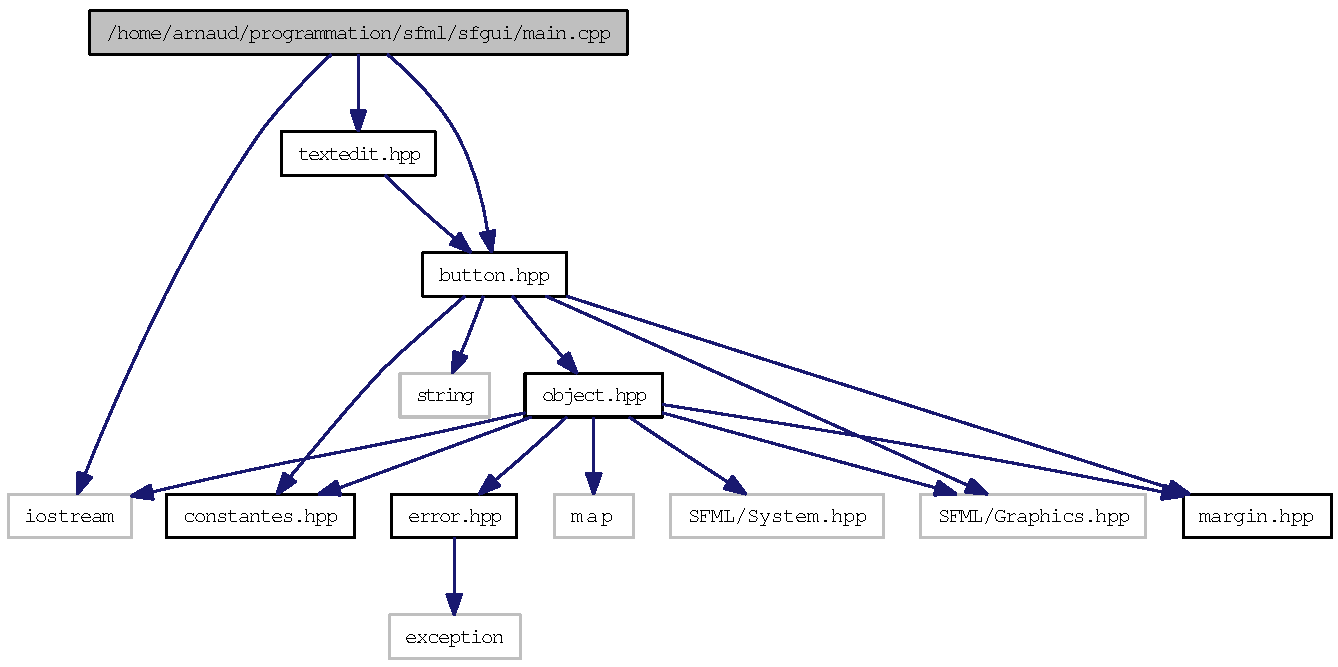
\includegraphics[width=339pt]{main_8cpp__incl}
\end{center}
\end{figure}
\subsection*{Functions}
\begin{CompactItemize}
\item 
sf::RenderWindow \hyperlink{main_8cpp_8991dd4eda96f401e33ee6ae24a46f0c}{App} (sf::VideoMode(800, 600, 32),\char`\"{}SFML GUI\char`\"{})
\item 
void \hyperlink{main_8cpp_fb33e4fdf2cfb177910c34fd0a19694d}{clickedCallBack} ()
\item 
void \hyperlink{main_8cpp_674037d7533f8891a97ed37d600aa1f9}{textChangeCallback} (std::string \&sr)
\item 
int \hyperlink{main_8cpp_e66f6b31b5ad750f1fe042a706a4e3d4}{main} ()
\end{CompactItemize}
\subsection*{Variables}
\begin{CompactItemize}
\item 
\hyperlink{classsfgui_1_1Button}{sfgui::Button} Sprite \& \hyperlink{main_8cpp_bcb2c6712035ac5e759315d67dced077}{App}
\end{CompactItemize}


\subsection{Function Documentation}
\hypertarget{main_8cpp_8991dd4eda96f401e33ee6ae24a46f0c}{
\index{main.cpp@{main.cpp}!App@{App}}
\index{App@{App}!main.cpp@{main.cpp}}
\subsubsection[App]{\setlength{\rightskip}{0pt plus 5cm}sf::RenderWindow App (sf:: {\em VideoMode}800, 600, 32, \/  \char`\"{}SFML GUI\char`\"{})}}
\label{main_8cpp_8991dd4eda96f401e33ee6ae24a46f0c}


\hypertarget{main_8cpp_fb33e4fdf2cfb177910c34fd0a19694d}{
\index{main.cpp@{main.cpp}!clickedCallBack@{clickedCallBack}}
\index{clickedCallBack@{clickedCallBack}!main.cpp@{main.cpp}}
\subsubsection[clickedCallBack]{\setlength{\rightskip}{0pt plus 5cm}void clickedCallBack ()}}
\label{main_8cpp_fb33e4fdf2cfb177910c34fd0a19694d}


\hypertarget{main_8cpp_e66f6b31b5ad750f1fe042a706a4e3d4}{
\index{main.cpp@{main.cpp}!main@{main}}
\index{main@{main}!main.cpp@{main.cpp}}
\subsubsection[main]{\setlength{\rightskip}{0pt plus 5cm}int main ()}}
\label{main_8cpp_e66f6b31b5ad750f1fe042a706a4e3d4}


\hypertarget{main_8cpp_674037d7533f8891a97ed37d600aa1f9}{
\index{main.cpp@{main.cpp}!textChangeCallback@{textChangeCallback}}
\index{textChangeCallback@{textChangeCallback}!main.cpp@{main.cpp}}
\subsubsection[textChangeCallback]{\setlength{\rightskip}{0pt plus 5cm}void textChangeCallback (std::string \& {\em sr})}}
\label{main_8cpp_674037d7533f8891a97ed37d600aa1f9}




\subsection{Variable Documentation}
\hypertarget{main_8cpp_bcb2c6712035ac5e759315d67dced077}{
\index{main.cpp@{main.cpp}!App@{App}}
\index{App@{App}!main.cpp@{main.cpp}}
\subsubsection[App]{\setlength{\rightskip}{0pt plus 5cm}{\bf sfgui::Button} Sprite\& App}}
\label{main_8cpp_bcb2c6712035ac5e759315d67dced077}


